\documentclass{standalone}
\usepackage{tikz}
\usetikzlibrary{arrows.meta}
\tikzset{label/.style = {inner sep=1pt, fill=white}}
%\tikzset{nd/.style={circle, inner sep=0pt}}
\tikzset{nd/.style={inner sep=1pt}}
\tikzset{>=Latex}
\tikzset{arc/.style = {->, semithick, >=Latex}}
\begin{document}
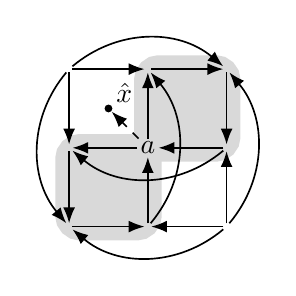
\begin{tikzpicture}

\draw [rounded corners, color = gray!30, line width = 10pt, fill] (1,1) to (1,2) to (2,2) to (2,1) to (1,1) to (0,1) to (0,0) to (1,0) to cycle;

    \node[nd] (1) at (0,0) {};
    \node[nd] (2) at (1,0) {};
    \node[nd] (3) at (2,0) {};
    \node[nd] (4) at (0,1) {};
    \node[nd] (5) at (1,1) {$a$};
    \node[nd] (6) at (2,1) {};
    \node[nd] (7) at (0,2) {};
    \node[nd] (8) at (1,2) {};
    \node[nd] (9) at (2,2) {};

    \node[nd, circle, inner sep= 1pt, fill] (x) at (0.5,1.5) {};
    \node at (0.7,1.7) {$\hat x$};

    \draw[arc,dashed] (5) to (x);
    
    \draw[arc] (4) to (1);
    \draw[arc] (3) to[in = -40, out = 220] (1);
    \draw[arc] (3) to[out = 50, in = -50] (9);
    \draw[arc] (8) to (9);
    \draw[arc] (5) to (8);
    \draw[arc] (5) to (4);
    
    \draw[arc] (7) to (4);
    \draw[arc] (7) to[in = 130, out = -130] (1);
    \draw[arc] (7) to (8);
    \draw[arc] (7) to[in = 140, out = 40] (9);
    \draw[arc] (1) to (2);
    \draw[arc] (3) to (2);
    \draw[arc] (2) to (5);
    \draw[arc] (2) to[in = -50, out = 50] (8);
    \draw[arc] (3) to (6);
    \draw[arc] (9) to (6);
    \draw[arc] (6) to (5);
    \draw[arc] (6) to[out = 220, in = -40] (4);

 \end{tikzpicture}
\end{document}